\begin{frame}	
	\frametitle{HTTP connection}
	\begin{columns}[t]
		\begin{column}[t]{0.5\linewidth}
			Http client:
			\begin{itemize}
				\item HttpURLConnection
				\item HttpAsnycTask class to run network operations independently from UI thread
				\item Implementation of an Android service to check requested video uploads
			\end{itemize}
		\end{column}
		\begin{column}[t]{0.5\linewidth}
			Class diagram:
			\begin{itemize}
				\item ...
			\end{itemize}
			
		\end{column}		
	\end{columns}	
\end{frame}

\begin{frame}	
	\frametitle{Camera}
	\begin{columns}[t]
		\begin{column}[t]{0.5\linewidth}
			Camera:
			\begin{itemize}
				\item No use of phone's default camera application.
				\item Own CameraActivity
				\item Use of Android's MediaRecorder.
				\item Storage of video files (.mp4 format) in the public directory for further usage. 
			\end{itemize}
		\end{column}
		\begin{column}[t]{0.5\linewidth}
			Class diagram:
			\begin{itemize}
				\item 
			\end{itemize}
			
		\end{column}		
	\end{columns}	
\end{frame}

\begin{frame}	
	\frametitle{Sensors}
	\begin{columns}[t]
		\begin{column}[t]{0.5\linewidth}
			Camera:
			\begin{itemize}
				\item Use of the accelerometer sensor
				\item Shake Detection
				\item Tilt Detection
				\item Preprocessed sensor data: ”Counter” value is send to the server.
				\item easy to add new sensors
			\end{itemize}
		\end{column}
		\begin{column}[t]{0.5\linewidth}
			Class diagram (Observer pattern): 
			\begin{itemize}
				\item ...
			\end{itemize}
			
		\end{column}		
	\end{columns}	
\end{frame}

\begin{frame}	
	\frametitle{SQLite database}
	SQLite database:
		\begin{itemize}
			\item Problem: coupling of actual video file and meta data persistently. 
			\item Use of Android's SQLite databases to have meta data persistently.
			\item Table: metadata
			\item Each filename is unique -> column filename be handled as a foreign key to the actual video file.
		\end{itemize}
\end{frame}

\begin{frame}	
	\frametitle{SQLite database}
		\begin{itemize}
			Table metadata: \hrule
			\begin{description}	
				\item[id] int primary key
				\item[filename] text
				\item[timestamp] text
				\item[duration] int
				\item[width] int
				\item[height] int
				\item[shaking] int
				\item[tilt] int
				\item[serverId] int
				\item[status] int
			\end{description}
		\end{itemize}
\end{frame}

\begin{frame}	
	\frametitle{User interface}
	\begin{columns}[t]
		\begin{column}[c]{.5\textwidth}
			\begin{figure}[!t]
				\centering
				\subfloat[Main]{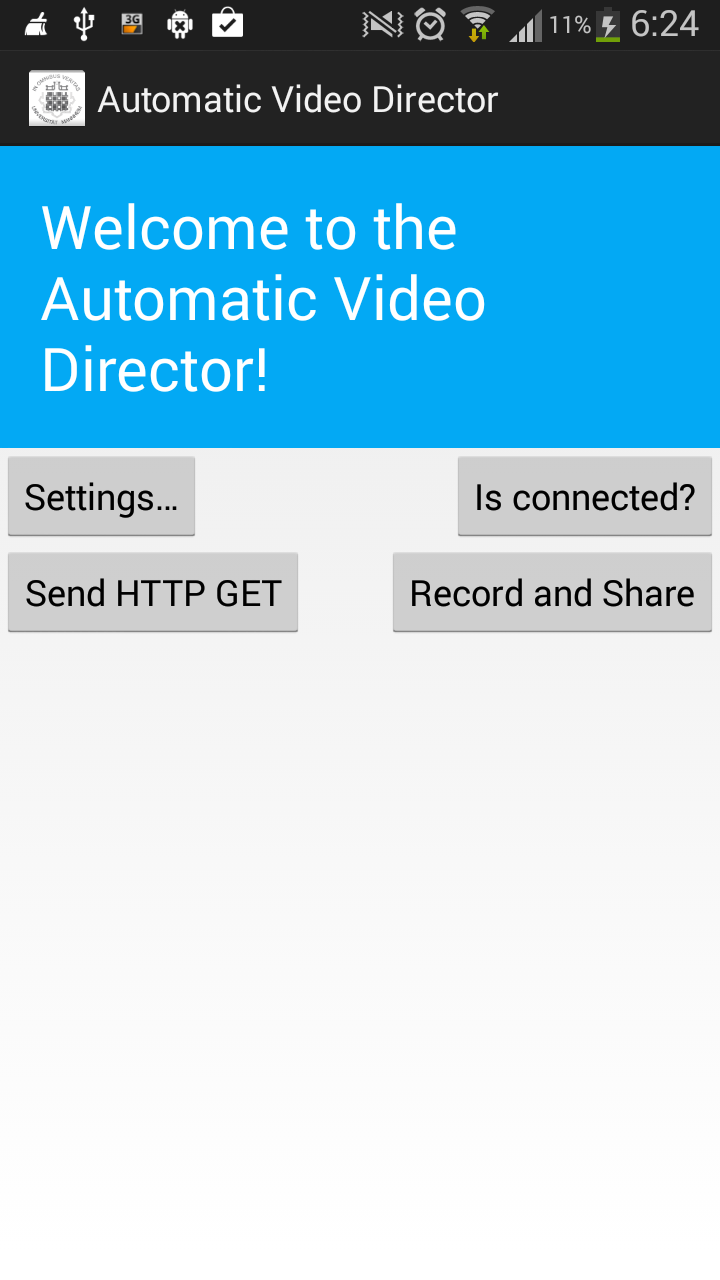
\includegraphics
						[width=.49\textwidth,height=.9\textheight,keepaspectratio]
						{ui_main.png}%
					\label{fig:ui_main}}
				\hfill
				\subfloat[Settings]{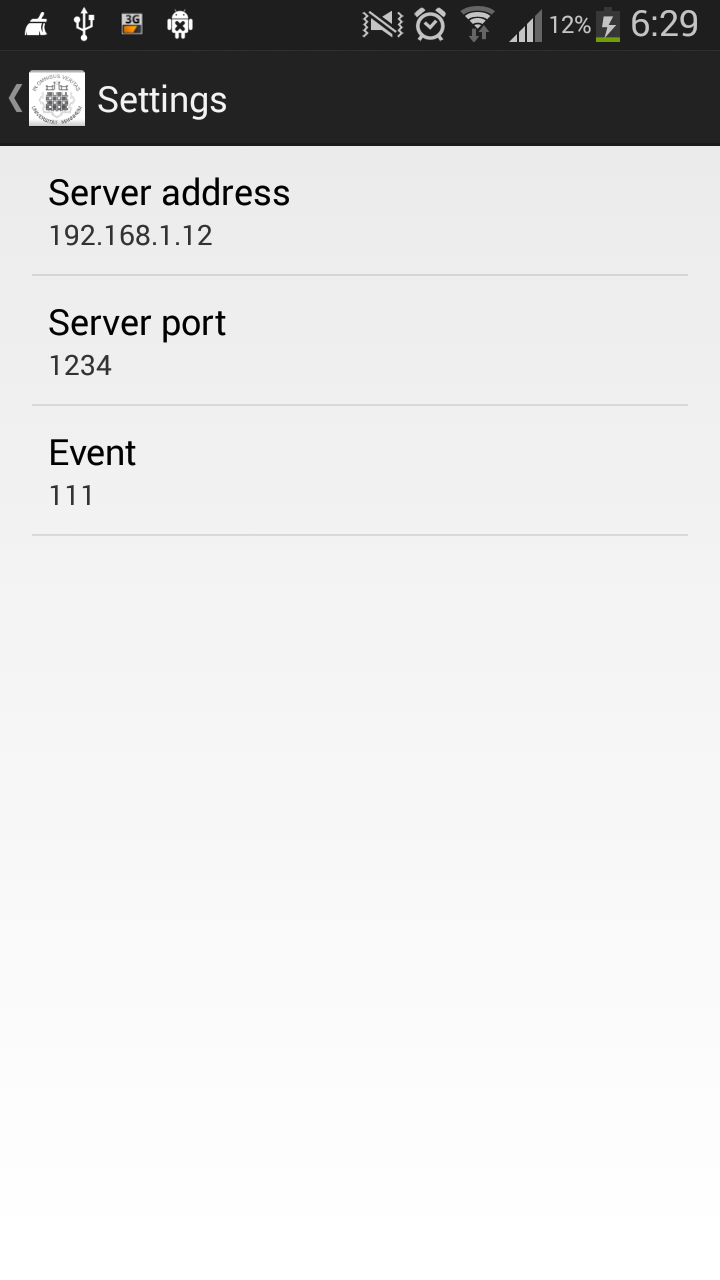
\includegraphics
					[width=.49\textwidth,height=.9\textheight,keepaspectratio]
					{ui_interface.png}%
					\label{fig:ui_settings}}
				\label{fig:ui_menu}
			\end{figure}
		\end{column}
		\begin{column}[c]{.5\textwidth}
			\begin{figure}[!t]
				\centering
				\subfloat[Camera]{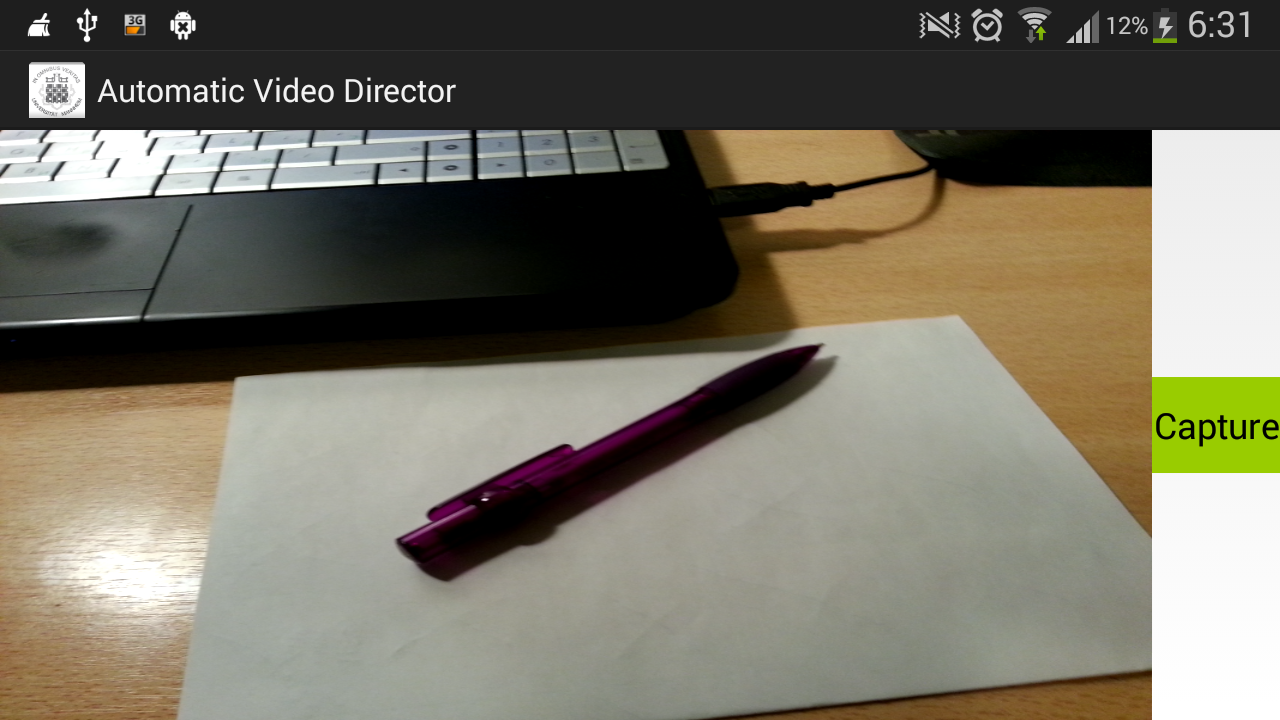
\includegraphics
					[width=\textwidth,height=.3\textheight,keepaspectratio]
					{ui_cam_green.png}%
					\label{fig:ui_cam_green}}
				\vfill
				\subfloat[Metadata upload]{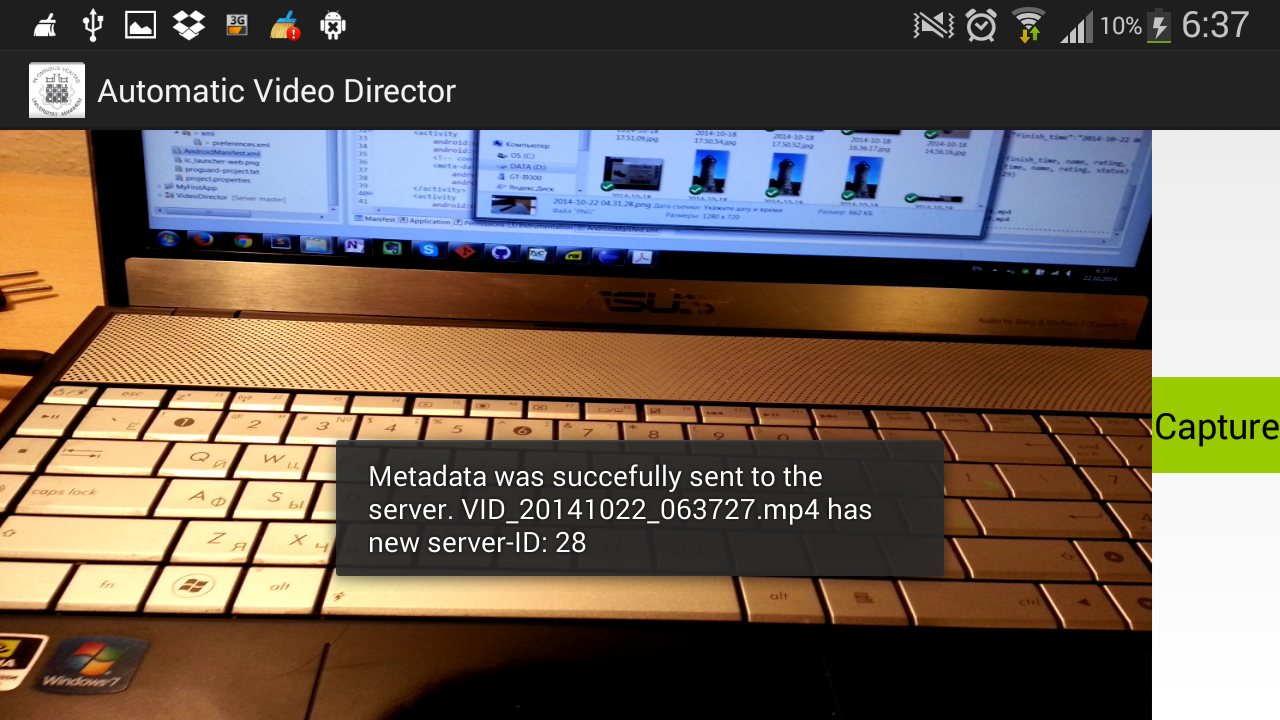
\includegraphics
					[width=\textwidth,height=.3\textheight,keepaspectratio]
					{ui_metadata.png}%
					\label{fig:ui_metadata}}
				\label{fig:ui_cam}
			\end{figure}
		\end{column}
	\end{columns}
\end{frame}